\documentclass[12pt]{article}
\usepackage[utf8]{inputenc}
\usepackage{mphysproject} % This includes graphicx, caption and geometry
\usepackage[block=space,bibencoding=utf8,style=phys,maxbibnames=6,giveninits=true]{biblatex}
\usepackage[toc,page]{appendix}
\usepackage{amsmath}
\usepackage{amsfonts}
\usepackage{physics}
\usepackage{siunitx}

\usepackage{hyperref}
\usepackage{cleveref}
\usepackage{float}
\usepackage{stackengine}
\usepackage{calc}
\usepackage{xcolor}

\usepackage[textsize=tiny]{todonotes}
\usepackage{lipsum}

\addbibresource{MPhys.bib}

\AtBeginEnvironment{appendices}{\crefalias{section}{appendix}}

% We often use underlines here
\stackMath
\newcommand{\suf}[2]{\stackunder[0.5pt]{\stackunder[1pt]{\ensuremath{#1}}{\rule{\widthof{\ensuremath{#2}}*\real{0.9}}{.1ex}}}{}}
\newcommand{\duf}[2]{\stackunder[0.5pt]{\stackunder[0.8pt]{\stackunder[1pt]{\ensuremath{#1}}{\rule{\widthof{\ensuremath{#2}}*\real{0.9}}{.1ex}}}{\rule{\widthof{\ensuremath{#2}}*\real{0.9}}{.1ex}}}{}}
\newcommand{\su}[1]{\suf{#1}{#1}}
\newcommand{\du}[1]{\duf{#1}{#1}}
\newcommand{\ssu}[1]{\scriptsize\su{#1}\normalsize}
\newcommand{\sdu}[1]{\scriptsize\du{#1}\normalsize}


\newcommand{\pp}{\ensuremath{\partial}}
\newcommand{\mgrad}{\ensuremath{\suf{\nabla}{K}\,}}
\newcommand{\QQ}{\ensuremath{\du{Q}}}
\newcommand{\NN}{\ensuremath{\su{N}}}
\newcommand{\MM}{\ensuremath{\su{M}}}
\newcommand{\EE}{\ensuremath{\du{E}}}
\newcommand{\PP}{\ensuremath{\du{\Pi}}}
\newcommand{\dudelta}{\ensuremath{\du{\delta}}}
\newcommand{\ddelta}[4]{\ensuremath{\delta_{#1#3}\delta_{#2#4} + \delta_{#1#4}\delta_{#2#3}}}

\newcommand{\FB}{\ensuremath{f_\text{bulk}}}
\newcommand{\FC}{\ensuremath{f_\text{comp}}}
\newcommand{\FU}{\ensuremath{f_\text{curv}}}

\newcommand{\onedot}{$\mathsurround0pt\ldotp$}
\newcommand{\cddot}{\mathbin{
    \vcenter{\baselineskip1ex \vspace{-0.1ex}\hbox{\onedot}\hbox{\onedot}}
}}

\begin{document}

\title{Normal Complex Tensor Order Parameter for Smectics in 3D}
\author{Jan Kocka}
\supervisor{Tyler N Shendruk}
%\date{1st January 2018}

\begin{abstract}
    \lipsum[10]
\end{abstract}

\maketitle

% This command introduces the Personal Statement: DO NOT REMOVE IT
\personalstatement
% Write PS here
\acknowledgments
% Write Acknowledgements here

\maintext

\section{Smectic Liquid Crystals}\label{sec:intro}
    \begin{figure}[t]
        \begin{center}
            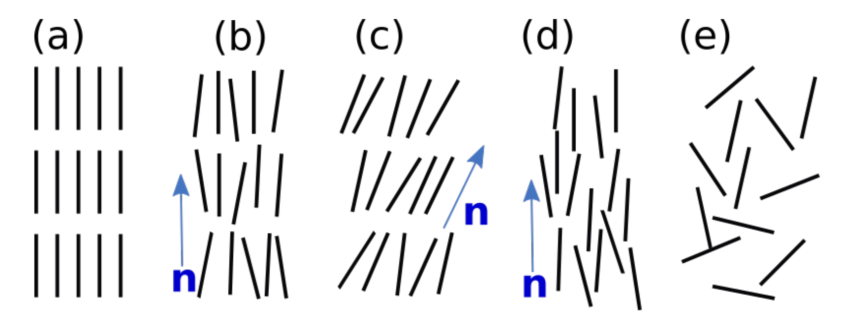
\includegraphics[width=0.95\textwidth]{figures/phases.pdf}
        \end{center}
        \caption{
            Illustrative structures of a substance made up from rod-like molecules.
            In order from (a) to (e) they are a fully crystalized phase, a smectic A, smectic C, nematic and an isotropic liquid.
            Image edited from\todo{cite jack's thesis}
        }\label{fig:phases}
    \end{figure}
    All, physicists will be well familiar with the ordered crystalline phase, in which the relative positions and possibly orientation of molecules is ordered, predictable and often repeating.
    Liquid crystals (LC) lay between this state and a typical liquid, some aspects of the phase are ordered, but others are not.
    This is best illustrated as a transition from an unordered (isotropic) liquid state as in \cref{fig:phases}.

    In an isotropic liquid the molecules have random, uncorrelated positions and orientations.
    Note that we talk about orientations, these are naturally only present if the molecules themselves are not spherical/symmetric.
    Depending on just how asymmetric they are they can have one or two orientation directions (in 3D), here we mainly look at rod-like molecules which have one, the axis of symmetry.
    The first step in ordering is usually a transition to a nematic liquid crystal in which the orientations of nearby molecules align, see \cref{fig:phases}.
    An important detail of nematic liquid crystals is that the constituent molecules are symmetric along their length as well (the is no head and tail) as this changes the physics, a nematic phase which does not have this symmetry is called a polar nematic.

    Next can come partial positional order, while different classification exist, in essence there are two ways this can happen in 3D.
    Either the symmetry is broken along one axis, these are the smectic phases, or along two in the columnar phases\cite{oswaldNematicCholestericLiquid2005}.
    In the columnar phases there remains only local one direction along which the system is not ordered.
    As such these phases are composed of separated columns of flowing liquid which are at ordered positions much like a 2D crystal.
    In the smectic phases, a broken symmetry along one axis results in a layered structure, the system is isotropic and flows within the layers but is organized along the layer normal.
    As such, smectics are fundamentally a layered phase, and that is what we focus on in this project, in essence we create a mesoscopic model for layering.

    There are various types of smectic phases, the simplest being the smectic A and C shown in \cref{fig:phases}.
    It is worth pointing out that the smectic layering coexists with a nematic order of the molecules.
    In smectic A phases the nematic orientation is always perpendicular to the layering, whereas in smectic C phases these are at an angle.
    Besides these there is a class of hexatic smectic phases, in which the molecules within layers locally arrange in a hexagonal lattice.
    However, while the lattice itself is only maintained for short distances, these local hexatic lattices have an orientation to them as well and this is aligned over large distances.
    Thus these feature yet more order than the smectic A and C phases, they include the B$_\text{hex}$ phase which has the nematic director perpendicular to the layering, along with the F and I phases which have an angle between the two.
    There are also smectic-like crystals which feature fully ordered often hexatic layers, among these are the B and E phases.
    For more details on these structures see \cite{oswaldNematicCholestericLiquid2005,oswaldSmecticColumnarLiquid2005,gennesPhysicsLiquidCrystals1995}.

    \todo[inline,size=\footnotesize]{This could be extended pretty much indefinitely, given the twist data we have perhaps the TGB would be the next thing worth mentioning}
    \todo[inline,size=\footnotesize]{Paragraph on why are they important/useful etc, the usual are soap, displays and hopefully something new? Bacteria! that might need a citation}

    The model presented in this thesis is in its early stages and so we mainly aim to capture the physics of the A and perhaps C phases.
    Though as we have extended the model into 3D it further highlighted that it captures the general concept of layers, and it does not currently have any concept of the underlying nematic order of smectics.
    There is a way to add that and it is perhaps the next step in developing this theory, however it also shows that the model might be used in other fields which require a mesoscopic model for layering.
    \todo{I don't like this paragraph but want to mention some of it somehow}

    \subsection{Ginzburg-Landau theory and the nematic \QQ\ tensor}\label{sec:GL_nem}
        Ginzburg-Landau theory is a powerful recipe to build phase transition theories, the work in this thesis being one of them.
        As such we start by introducing these on the example of an isotropic liquid to nematic LC transition for two reasons.
        Because nematic order often underlays smectic order and so the two need to be considered simultaneously, and because the \QQ\ tensor theory for nematics has heavily inspired the \EE\ tensor theory for smectics this thesis is based on.

        \subsubsection{The order parameter}\label{sec:nem_op}
        The central concept of Ginzburg-Landau theory is the order parameter, this is usually some mathematical object such as a scalar, vector or tensor that has known values for each of the phases and varies in between them in mostly a smooth manner.
        If a single order parameter is used to describe the entire system in question as a whole, it is a Landau theory, one can extract useful information using this alone.
        However, Ginzburg-Landau theory goes a step further and promotes the order parameter to a field.
        This way one may have a part of the system be in one phase and a different part in the other.

        Going back to our example of a nematic LC, this order parameter needs to capture how aligned the molecules are at each point, accounting for the nematic symmetry.
        The way to do this is using the \QQ\ tensor which can be obtained from a system of discrete molecules via
        \begin{equation}
            \du{Q}_\text{mol} = \su{N}_\text{mol}\su{N}_\text{mol} - \frac{\dudelta}{d}
        \end{equation}
        where $\su{N}_\text{mol}$ is a unit vector denoting the orientation of a molecule, $\dudelta$ the identity and $d$ the dimensionality of the system (2 or 3).
        Throughout this thesis we use underlines to denote tensors, the number of underlines being their rank, further if two tensors appear side by side then it means a dyadic/tensor product and any contractions are denoted by dots \nolinebreak $\cdot$ (the contraction order usually does not matter).
        Note that $\du{Q}_\text{mol}$ immediately satisfies the nematic symmetry of to $\su{N}_\text{mol}$ being the same as $-\su{N}_\text{mol}$.
        So each molecule has a $\du{Q}_\text{mol}$ and we take a local average of these to arrive at the tensor field \QQ\ (taking these local minima numerically can be quite tricky).
        Given the form of \QQ\ we can then reexpress it as the following
        \begin{equation}\label{eq:Qua}
            \du{Q} = S\qty(\su{N} \su{N} - \frac{\dudelta}{d}) \color{gray} + \text{possibly more terms, ignore for simplicity here} \normalcolor
        \end{equation}
        where $S$ is a number between 0 and 1, $\su{N}$ is a unit vector and both are fields along with \QQ.
        From there it is easy to see that an isotropic liquid would have $\du{Q} = S = 0$ and a fully nematic one would have $S = 1$ and \NN\ be the orientation of the phase.
        From this it is clear that $\du{Q}$ is a valid order parameter to describe the isotropic to nematic transition, it is in fact the most widely used such parameter due to it respecting the orientational symmetry.

        \subsubsection{The free energy density and deformations}
        Now that we have an order parameter, the next step in forming a Ginzburg-Landau theory is to find a suitable free energy, physics then follow through minimization of it.
        This will be a volume integral of a free energy density $f(\su{r})$ over the system and potentially surface contributions $\mathcal{F}(\su{r})$
        \begin{equation}
            F = \int f(\su{r}) dV + \int \mathcal{F}(\su{r}) dS
        \end{equation}
        though the surface is often dealt with separately.
        $f(\su{r})$ should only depend on the order parameter \QQ\ and elastic constants, it must be local, and crucially it must maintain any symmetries of the system\cite{kardarStatisticalPhysicsFields2007,reichlModernCourseStatistical2016}.
        This can be done in two ways, if one know the underlying microscopic interactions then these can be coarse-grained to obtain $f(\su{r})$.
        However, this can be very difficult or not possible at all, and one might not know all the microscopic interactions.
        This is where the power of Ginzburg-Landau theories lays as one may instead start taking all possible symmetry-allowed terms of $f(\su{r})$ increasing in power of the order parameter and stop once all the physics is captured\todo{could use a citation, got this from StatPhys notes}.
        % This approach will only be valid near the critical point and under 

        In the example of \QQ, that already contains the $\su{N} \leftrightarrow -\su{N}$ symmetry and the bulk free energy density (which does not account for gradients) should only depend on $S$ as it should be the same regardless of the orientation direction.
        As such we have $f_\text{bulk}(\su{r})$ being a power series of $S$ and given \cref{eq:Qua} that translates to a series of suitably contracted terms of \QQ.
        Generally, the following form is used
        \begin{equation}\label{eq:Qfbulk}
            f_\text{bulk}(\su{r}) = \frac{a}{2} \Tr(\du{Q}^2) - \frac{b}{3} \Tr(\du{Q}^3) + \frac{c}{4} \Tr(\du{Q}^2)^2 = \frac{a}{2} Q_{ij}Q_{ij} - \frac{b}{3} Q_{ij}Q_{jk}Q_{ki} + \frac{c}{4} Q_{ij}Q_{ij}Q_{kl}Q_{kl}
        \end{equation}
        where $b$ and $c$ are positive constants and $a$ can have either sign, the terms correspond to $S^2, S^3$ and $S^4$ terms\cite{brayTheoryPhaseOrdering1993,luckhurstBiaxialNematicLiquid2015}.
        The repeated indices in the second form of \cref{eq:Qfbulk} being Einstein summation indices which are assumed throughout this thesis unless otherwise specified.
        This form can have one or two minima for $S\geq0$, this is determined by the coefficients which are set relative to a critical temperature or concentration.
        Without going through the details, generally one takes enough terms to allow for a suitable number of minima (each of which corresponds to a stable or metastable phase), then one extra term with a positive coefficient is added to make sure that $f_\text{bulk}(\su{r})$ keeps growing at very large order parameter.

        However, $f_\text{bulk}(\su{r})$ does not account for any deformation energy costs, which is naturally a key ingredient to describing a system.
        To add these we introduce terms to $f(\su{r})$ which depend on the gradients of the order parameter.
        This gets more complex, though the same rule still applies, take as many allowed terms in increasing powers of the order parameter and \mgrad\ as is needed.
        However, here finding the correct form can get tricky and one generally starts considering specific geometries of the system and what their deformation terms should be like.
        If one is to work analytically or on a constrained system, it might also be that certain terms are negligible and others are not, as such, which terms are used varies in literature.

        \begin{figure}[t]
            \begin{center}
                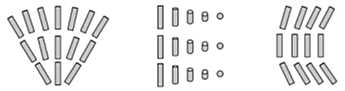
\includegraphics[width=0.6\textwidth]{figures/nematic_deformations.jpg}
            \end{center}
            \caption{
                Diagrams of the splay, twist and bend nematic deformation types respectively.
                Image taken from \cite{suryantariImageFeatureExtraction2019}.
            }\label{fig:nem_deform}
        \end{figure}

        For the nematic case, in the simplest case of constant $S$ but varying \NN\ we get the Frank-Oseen deformation energy terms\cite{brayTheoryPhaseOrdering1993,frankLiquidCrystalsTheory1958,gennesPhysicsLiquidCrystals1995}
        \begin{align}
            K_1 (\mgrad \cdot \su{N})^2 && K_2 (\su{N} \cdot \mgrad \times \su{N})^2 && K_3 (\su{N} \times \mgrad \times \su{N})^2
        \end{align}
        where the $K$s\todo{is this okay?} are positive elastic constants.
        These three terms correspond to three type of deformation of the director \NN: splay, twist and bend respectively, as shown in \cref{fig:nem_deform}.
        Adapting these to be in terms of \QQ\ has proven difficult, first attempted by de Gennes\cite{gennesPhysicsLiquidCrystals1995} using the terms
        \begin{align}
            L_1Q_{ij,k}Q_{ij,k} && L_2Q_{ij,j}Q_{ik,k} && L_4\epsilon_{ijk}Q_{il}Q_{jl,k}
        \end{align}
        with $L$s being elastic constants and $\epsilon$ the Levi-Civita tensor.
        However, these have later been shown to imply $K_1 = K_3$\cite{lubenskyMolecularDescriptionNematic1970}, which is contradicted by experiment.
        Since then additional terms have been added to account for this\cite{longaExtensionLandauGinzburgdeGennes1987} though that is going beyond the scope of this summary.
        What is worth noting however is the one constant approximation, where all the $K$ elastic constants are taken to be equal which leads to all the terms collapsing to
        \begin{equation}
            L_1 Q_{ij,k}Q_{ij,k}
        \end{equation}
        While this is the simplest possible approximation, it has been used widely for both numerical and analytical studies, and historically it has been the starting point before the different terms have all been discovered.\todo{Not sure the second part is true...}
        In many ways it highlights the idea of Ginzburg-Landau theory in that it is the simplest possible term one can construct using \QQ\ and \mgrad\ and it captures all the possible deformation terms.
        In the work on smectics presented in this thesis we start from a similar approximation, still using it but also trying to go a step beyond and develop more specific terms which collapse to the approximation.


        \subsubsection{Biaxial nematics and \QQ}\label{sec:Q_biax}
        There is one additional bit of complexity worth introducing and that is biaxiality of nematics.
        We have been talking about the orientation of molecules as being a single direction, which is correct for rod-like molecules.
        However, if the molecules are completely asymmetric then there can be order in two perpendicular directions.
        Say we have long cuboid molecules, they can first order by aligning their longest axes and then also rotate around those axes so that the next longest axes also align.
        The same applies to any asymmetrical shaped molecules in 3D (this cannot happen in 2D as there are less orientational degrees of freedom).

        It demonstrates the power of \QQ\ that we can still use it to describe this dual order, we can still calculate it exactly the same way through $\du{Q}_\text{mol}$ and \QQ\ will still be symmetric and traceless, however we now allow it to take the more general form
        \begin{equation}\label{eq:Qbiax}
            \du{Q} = S_1\qty(\su{N} \su{N} - \frac{\dudelta}{d}) + S_2\qty(\su{M} \su{M} - \frac{\dudelta}{d})
        \end{equation}
        where $\su{N}$ and $\su{M}$ are mutually orthogonal unit vectors which describe the directions of the two orders, with $S_1$ and $S_2$ acting as their corresponding order parameters.

        This more general type of nematic order comes with many complications especially when it comes to the free energy forms as it is difficult to separate the two orders contained in \QQ.
        However, it has been extensively studied during the last decades with fascinating phases being used including those of banana shaped molecules\cite{luckhurstBiaxialNematicLiquid2015,kumarBiaxialityNematicSmectic2017,kimCurvaturesSmecticLiquid2018}.

        % \todo[inline,size=\footnotesize]{This needs more, cite/use\cite{luckhurstBiaxialNematicLiquid2015} mention how final states for uniaxial nematics have a uniaxial Q even when using eq above, aka S2 = 0, though I need a thing to cite for that}

    \subsection{Describing smectics\cite{oswaldSmecticColumnarLiquid2005}}\label{sec:degennes}
        Fundamentally, the layered positional order corresponds to a wave-like density fluctuation.
        Following \cite{oswaldSmecticColumnarLiquid2005} in the approach suggested by de Gennes, if we first only consider a single wave throughout the entire system, then the density field is
        \begin{equation}\label{eq:density_base}
            \rho(\su{r}) = \rho_0 + \rho_1\cos(\su{q_0}\cdot\su{r} + \phi) = \rho_0 + \Re(\rho_1 e^{i(\ssu{q_0} \cdot \ssu{r} + \phi)})
        \end{equation}
        where $\rho_0$ is the average density, $\rho_1$ is the wave amplitude, $\phi$ an arbitrary phase (determined by boundary conditions) and $\su{q_0}$ its wavevector containing both the wave direction ($\su{N} = \frac{\ssu{q_0}}{q_0}$ being the layer normal, the smectic director) and spacing ($\frac{2\pi}{q_0}$).
        This is a very simple start, however already one can take $\rho_1$ as an order parameter (not a field here, making this a Landau theory) with 0 corresponding to no wave and so an isotropic liquid.
        To then build a bulk free energy in terms of $\rho_1$ we need to identify any symmetries.
        The only relevant symmetry here is that of $\rho_1 \leftrightarrow -\rho_1$ as such a change only leads to a change in the phase $\phi$ which is not a physical change.
        Such a change would keep the same wave amplitude and spacing and as such the smectic phase is unchanged and so should be its free energy.
        The implication of this is that the free energy may only have even power terms of $\rho_1$ becoming
        \begin{equation}
            F_\text{bulk} = \frac{A}{2}\rho_1^2 + \frac{B}{4}\rho_1^4 + \frac{C}{6}\rho_1^6 + \cdots
        \end{equation}
        with $A, B, C$ being constants which determine the order of the isotropic-smectic phase transition\cite{oswaldSmecticColumnarLiquid2005}.

        The natural next step is to promote $\rho_1$ to a field and the free energy to a free energy density, this leads to equivalent bulk terms but also deformation terms.
        In that case the layering direction and spacing is uniform throughout the system, however the ordering can be perfectly smectic or perfectly isotropic in different areas.
        To account for local changes to layering direction and spacing one must allow some part of the phase of \cref{eq:density_base} to change in space.

        Different choices can be made in that regard, the first and most commonly used being to keep $\su{q_0}$ constant but make $\phi$ a field.
        This allows the layers to locally contract, dilate and tilt in small magnitudes as the phase changes through $\phi$.
        This is a particularly good approach to study near equilibrium configurations, their stability and energetics as it contains enough information yet is simple enough for analytical work.
        Going a step  further, $\su{q_0}$ need not be constant throughout the system as long as we keep it fixed in time.
        This way more interesting geometries can be studied through an imposed $\su{q_0}$ and solving for $\rho_1$ and $\phi$.

        It is worth elaborating a little on what exactly $\phi$ means once we have made it a field.
        It is difficult to quantify how exactly it may alter the layering direction and so we do not discuss that here, however there is a clear correspondence between gradients in $\phi$ and contractions and dilations.
        For simplicty, consider a 1D system with $\phi = s x$ where $s$ is a constant gradient, then clearly we have $e^{i(q_0 x + s x)} = e^{i(q_0 + s) x}$ or in other words we simply have a modified wavelength of $\frac{2\pi}{q_0 + s}$.
        For a more complex example see \cref{fig:gradphi} where we have a spherically symmetric setup of $\su{q_0} = \frac{2\pi}{2\si{L}} \hat{\su{r}}$ with \si{L} being an arbitrary unit of length and
        \begin{equation}\label{eq:gradphi_phi}
            \phi(\su{r}) = \begin{cases} 0 & \qq{if} r \leq 5\si{L} \\ s(r - 5\si{L}) & \qq{if} r \geq 5\si{L} \end{cases}
        \end{equation}
        In other words, $\phi$ has a constant gradient of $s$ in the layering normal direction for $r\geq5\si{L}$ which results in a constant change to layer spacing.
        The key point here being that gradients of $\phi$ in the direction of layering correspond to contractions and dilations.

        \begin{figure}[t]
            \begin{center}
                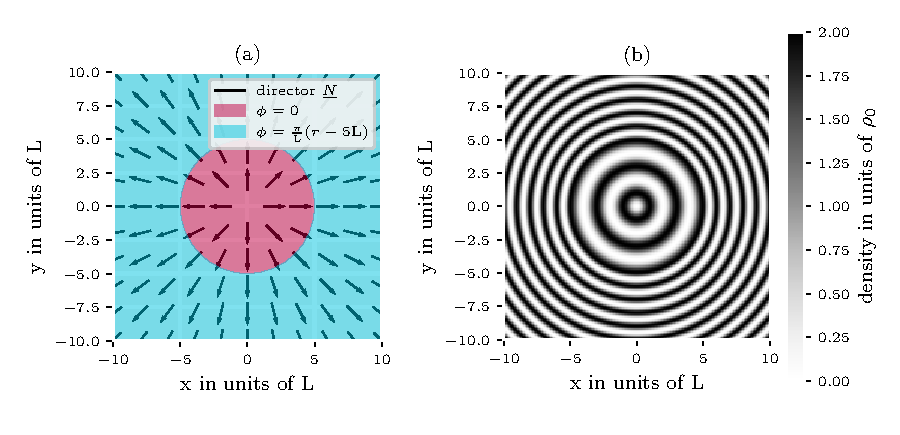
\includegraphics{figures/misc/wave_phi_example.pdf}
            \end{center}
            \caption{
                Diagrams of how \cref{eq:density_base} behaves for a 2D, spherically symmetric system with a non-uniform but fixed $\su{q_0} = \frac{2\pi}{2\si{L}}\hat{\su{r}}$, constant $\rho_1 = \rho_0$ (so a fully smectic phase) and $\phi$ given by \cref{eq:gradphi_phi} with $s=\frac{\pi}{\sii{L}}$.
                \si{L} here is an arbitrary unit of length.
                (a) shows the layer normal direction \NN\ and highlights the two zones for $\phi$.
                (b) shows the resulting density having constant wavelengths of $2\si{L}$ and $\frac{2\pi}{\frac{2\pi}{2\si{L}}+\frac{\pi}{\si{L}}} = 1\si{L}$ in each of the zones from (a).
            }\label{fig:gradphi}
        \end{figure}

        In these approaches a complex order parameter $\psi=\rho_1e^{i\phi}$ is used to simplify \cref{eq:density_base} to $\rho(\su{r}) = \rho_0 + \Re(\psi(\su{r}) e^{i\ssu{q_0}\cdot\ssu{r}})$, this is known as the de Gennes order parameter.
        In essence, it replaces the degrees of freedom of two real parameters by a single complex one.
        It is using this theory that de Gennes has demonstrated an analogy between smectic liquid crystals and superconductors\cite{degennesAnalogySuperconductorsSmectics1972}, a particularly fruitful contribution leading to better understanding of the twist-grain boundary phase\cite{lubenskyTwistgrainboundaryPhasesNematic1990} among others.

    \subsection{Smectic (and nematic) defects}

    \subsection{Limitations of $\psi$ and the $\su{N} \leftrightarrow -\su{N}$ symmetry}\label{sec:pevnyi}
        The theoretical framework described in \cref{sec:degennes} has been very successfully used since the second half of the 20th to understand many of the smectic and other liquid crystalline phases\todo{needs citations...}.
        However, it also comes with some significant shortcomings, two of which have been highlighted by Pevnyi, Selinger and Sluckin in 2014\cite{pevnyiModelingSmecticLayers2014} and which have sparked renewed interest in smectic studies.
        As a response a new smectic order parameter \EE\ has been developed along with a corresponding free energy form by Paget et al\cite{pagetComplexTensorsSimple2023,pagetSmecticLayeringLandau2022,pagetComplextensorTheorySimple2023} and this thesis continues that work.

        The main issue arises when studying the dynamics of more complex systems as when studying a how different domains may form during the isotropic to smectic transition and how they then merge and defects annihilate\cite{ambrozicAnnihilationEdgeDislocations2004,abukhdeirDefectKineticsDynamics2008}.
        In these cases the mentioned approach of keeping $\su{q_0}$ fixed and only working with $\rho_1$ and $\phi$ from \cref{eq:density_base} cannot work.
        In theoretical studies this can often be circumvented by separating the system into domains manually, however this is not feasible for numerical studies.
        If one is to model such a complex system using a single set of fields, a slightly different complex order parameter is used which replaces all the degrees of freedom from \cref{eq:density_base}\cite{mukherjeeSimpleLandauModel2001,mukherjeeAdvancesIsotropicSmectic2021}.
        Mathematically this is equivalent to setting $\su{q_0} = 0$ with us now having
        \begin{equation}\label{eq:density_pevnyi}
            \rho(\su{r}) = \rho_0 + \Re(\psi(\su{r}))
        \end{equation}
        and $\phi$ carrying all of the phase information including the layering direction and spacing.
        The layering wavevector can then be recovered via $\su{q_0} = \mgrad \phi$ and so the layering normal direction is $\su{N} = \frac{\mgrad \phi}{|\mgrad \phi|}$.

        \begin{figure}[t]
            \begin{center}
                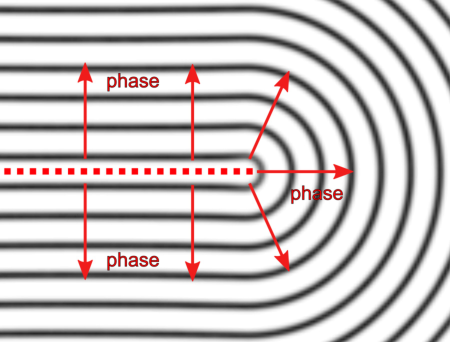
\includegraphics[width=0.4\textwidth]{figures/pevnyi.pdf}
            \end{center}
            \caption{
                Diagram of a $+\frac{1}{2}$ defect in the smectic phase to demonstrate the double-valuedness of the de Gennes complex order parameter, taken from \cite{pevnyiModelingSmecticLayers2014}.
                Black lines correspond to smectic layers, red arrows point in the direction of increasing (or decreasing, this is a choice) $\phi$.
                Dotted red line is where the gradient of $\phi$ discontinuously changes (this can be chosen to be elsewhere) even though the layering there is uniform.
            }\label{fig:pevnyi}
        \end{figure}

        This is the order parameter that Pevnyi et al discuss and the main problem they bring up is that $\psi$ is fundamentally double-valued, or in other words ill-defined.
        Why this is perhaps best shown on the example of a smectic system with a $+\frac{1}{2}$ defect, as in \cref{fig:pevnyi}.
        In order to obtain such layering in the model of \cref{eq:density_pevnyi} there must be an increasing or decreasing $\phi$ perpendicular to the layering.
        Now consider it is increasing downwards in the bottom half of \cref{fig:pevnyi}, then as $\phi$ ought to be smooth in the defect free region to its right and around the defect, we end up with an upwards increasing $\phi$ in the upper region of \cref{fig:pevnyi}.
        This then gives a line of a discontinuous change in $\su{N} = \mgrad \phi$ in the middle left, along the highlighted line, which is also defect free and so any fields should be changing smoothly.

        Ultimately this double-valuedness is a result of the smectic $\su{N} \leftrightarrow -\su{N}$ symmetry as layering upwards and downwards is physically the same.
        This is exactly what we see in the left part of \cref{fig:pevnyi} where we get \NN\ pointing downwards in the bottom half and upwards in the upper half.
        The problematic middle line is unclear, however in a physical sense both directors are equivalent and the phase is continuous.
        This problem is not a purely formal one either, unless accounted for it leads to unphysical line defects appearing between point defects\cite{pevnyiModelingSmecticLayers2014} and associated unphysical energy costs.
        This is the key problem that \EE\ theory aims to solve.

    \subsection{Other approaches and recent smectic results}\label{sec:sm_other}
        Naturally, other approaches to these problems have been developed as well.
        Pevnyi et al themselves suggest working with the density directly instead of using a coarse-grained mesoscopic order parameter\cite{pevnyiModelingSmecticLayers2014,xiaStructuralLandscapesGeometrically2021,farrellFiniteelementDiscretizationSmectic2023,xiaSimpleTensorialTheory2024}.
        There $\delta\rho(\su{r}) = \rho(\su{r}) - \rho_0 = \Re(\psi(\su{r}))$ is used as the order parameter and a free energy constructed in terms of it.
        In essence this resolves the symmetry problem by switching to a more microscopic picture whereas \NN\ only appears through $\delta\rho$ as a macroscopic variable.
        Of course the free energy must be carefully crafted so that layering does appear, one way to do this is to relate $\delta\rho$ to $\psi$ and use the same free energies that have been developed for $\psi$\cite{pevnyiModelingSmecticLayers2014}.

        Another benefit of this microscopic treatment is that individual layers in the smectic are resolved, unlike in the approaches using $\psi$ where the focus is on the degree of ordering and layer normal direction.
        This is a notable feature as precise layer positioning plays a role in dislocation defects \todo{cref to figure of defect} and it also allows to obtain the preferred layer spacing $q_0$ through simulations instead of considering it as an outside parameter like in most $\psi$ based approaches.
        % The same also applies to $\rho_1$ which can be obtained from simulaltions as opposed to when using $\psi$
        % and the same applies to $\rho_1$ where often $|\psi|$ is taken in the range 0 to 1 (for a fully isotropic and smectic systems respectively) and then scaled by $\rho_1$ (or in fact $\rho_0$) as a physical parameter.

        However, the microscopic nature of this density-based approach is also its largest limitation at it severely limits the size of systems that can be numerically solved for.
        Given that the individual layers need to be captured, in a naive numerical solver many numerical grid points are needed per wavelength $\frac{2\pi}{q_0}$.
        % Given that the individual layers need to be captured, in a naive numerical solver at least on the order of 5 to 10 numerical grid points would be needed per wavelength $\frac{2\pi}{q_0}$.
        In a comparable study using a mesoscopic order parameter only a single grid point might well be sufficient, even less in more uniform areas and perhaps more near defects.

        Additionally, a completely different approach to modelling smectics has also been developed since the end of the last century based on dynamical density functional theory and phase field crystal methods\cite{lowenPhasefieldcrystalModelLiquid2010,elderModelingElasticPlastic2004,achimStabilityLiquidCrystalline2011,vitralPhasefieldModelWeakly2021,nestlerActiveSmecticsSphere2023}.
        This is a rather complex approach which starts at the individual particles, their positions, orientations and interactions and coarse-grains these.
        As such these at a fundamental level describe a more general liquid crystal system of non-spherical (mainly rod-like) particles which may have both nematic and smectic order.
        In the methods of \cite{lowenPhasefieldcrystalModelLiquid2010} one ends up with three fields: the particle density field $\psi_1$, a nematic order parameter $\psi_2$ and the nematic director field $\su{u_0}$.
        The nematic order fields $\psi_2$ and $\su{u_0}$ vaguely corresponding to the $S$ and \NN\ parameters from \cref{sec:nem_op}.

        This is a promising method, in particular when considering its generality when it comes to different types of order, physical insight and mathematical rigour.
        However, for simulating large mesoscopic systems it shares the same limitations of the density based methods using $\delta\rho$.
        Similarly to those, the smectic ordering is fully captured by a density field (though how that is done is very different) and so it is a microscopic picture of the smectic which limits the scope of numerical simulations.

        \todo[inline,size=normalsize]{Maybe add something about Monderkampf simulation results?}

\section{Introduction to \EE\ Theory}\label{sec:Eintro}
    In this chapter we introduce \EE\ theory, a Ginzburg-Landau theory for smectic liquid crystals and perhaps other layered systems as developed by Paget, Shendruk et al\cite{pagetComplexTensorsSimple2023,pagetSmecticLayeringLandau2022,pagetComplextensorTheorySimple2023} and continued as a part of this thesis.
    Firstly, to revise the main objectives and motivations for \EE.
    The goal is to develop a mesoscopic order parameter of layering that is suitable for large numerical simulations.
    Mesoscopic meaning that it does not resolve individual layers but only their overall ordering, direction and spacing.
    To start, the focus is in particular on the smectic A and perhaps C phases.
    It follows in the approach of de Gennes by using a complex number field, however it must account for the $\su{N} \leftrightarrow -\su{N}$ symmetry in order to avoid unphysical defects.

    As we continue in the spirit of the de Gennes parameter, we start at the density wave equation
    \begin{equation*}
        \rho(\su{r}) = \rho_0 + \Re(\rho_1 e^{i(\ssu{q_0} \cdot \ssu{r} + \phi)}) \tag{\ref{eq:density_base} revisited}
    \end{equation*}
    with the layer normal being $\su{N} = \frac{\ssu{q_0}}{q_0}$.
    We want to build a model capable of describing complex smectic systems, and so we require full flexibility in both the wave amplitude and phase throughout space.
    However, unlike previously when the entire phase of \cref{eq:density_base} was replaced by a phase field $\phi(\su{r})$, here we keep both $\su{q_0}$ and $\phi$ as they are and make them both fields.
    Specifically, we take the magnitude of the wavevector $q_0$ to be a constant physical parameter (perhaps dependent on temperature or other macroscopic variables, though that is not considered here) but allow its direction \NN\ to vary in space.

    So we have three independent fields $\rho_1(\su{r})$, $\su{N}(\su{r})$ and $\phi(\su{r})$, and we would like to form a complex order parameter as before, though to be completely clear it is worth noting the units.
    $\su{N}(\su{r})$ is a dimensionless unit vector, $\phi(\su{r})$ a dimensionless phase but $\rho_1(\su{r})$ has units of density whereas we would like the complex order parameter be dimensionless.
    To achieve that we define $\psi(\su{r}) = \frac{\rho_1(\ssu{r})}{\rho_1}e^{i\phi(\ssu{r})}$ where $\rho_1$ is a constant with units of density that defines the amplitude of the density wave for a fully ordered smectic.
    This leads to
    \begin{equation}
        \rho(\su{r}) = \rho_0 + \rho_1 \Re(\psi(\su{r}) e^{i q_0\ssu{N}(\ssu{r}) \cdot \ssu{r}}) = \rho_0(1 + \frac{\rho_1}{\rho_0} \Re(\psi(\su{r}) e^{i q_0\ssu{N}(\ssu{r}) \cdot \ssu{r}}))
    \end{equation}
    where all the fields are written explicitly, $\psi(\su{r})$ is a dimensionless complex order parameter with magnitude between 0 and 1 and $\rho_0$, $\rho_1$ and $q_0$ are all physical constants defining what a smectic phase would look like on a microscopic level, if one was to make that connection.
    For a further, but reasonable, simplification we may use $\rho_1 = \rho_0$ which is the largest value it may take and it corresponds to a fully smectic phase having the density $\rho(\su{r})$ reach zero in the layer gaps.

    Now we are left with a complex field $\psi(\su{r})$ and a unit vector field $\su{N}(\su{r})$, from now on the explicit field notation will be dropped.
    As established, $|\psi|$ describes how smectic or layered a system is and both \NN\ and $\phi$ influence the phase.
    There is clearly a redundancy between the two, however both are necessary.
    We want a direct way to access \NN\ in order to account for the $\su{N} \leftrightarrow -\su{N}$ symmetry, however using only it would not allow any layer compressions or dilations, and so we must also allow an additional phase $\phi$.
    However, as $\phi$ can also affect the layering direction if it has large gradients in the directions perpendicular to \NN, it is worth noting that the layering direction may be offset from \NN.
    However, in our interpretations we still think of \NN\ as representing the layering direction and gradients of $\phi$ the compressions and dilations (see \cref{fig:gradphi}), this is valid as long as $\phi$ varies slowly compared to \NN\ which is the case in our simulations.

    Now that we have our building blocks ready, we finally need to take account of the $\su{N} \leftrightarrow -\su{N}$ symmetry.
    This is done in analogy to the nematic \QQ\ (\cref{sec:nem_op}) and we define a new order parameter, the \EE\ tensor, as
    \begin{equation}\label{eq:Eua_def}
        \du{E} = \psi \qty(\su{N}\su{N} - \frac{\du{\delta}}{d})
    \end{equation}
    where $d$ is the number of physical dimensions we consider.
    Just as in the nematic case this immediately enforces the $\su{N} \leftrightarrow -\su{N}$ symmetry and in addition it bundles all of our order parameter fields together.
    This has not been discussed before, but for numerical simulations this comes with another significant advantage as it allows numerical melting in defects.
    To see that consider say an aster-like defect with \NN\ pointing outwards from a point where the phase becomes an isotropic liquid.
    In this system the director \NN\ (and $\phi$ as well) is not well-defined at the point defect and so trying to calculate in numerically leads to issues.
    However, as $|\psi|$ goes to zero at the defect point, so does \EE\ and so it is clearly defined and calculable everywhere.

    As Paget et al note, the tensor field constructed in \cref{eq:Eua_def} is by definition globally gauge invariant (a global shift in phase has no physical effect) and the complex tensor $\du{E}(\su{r})$ at any point is by construction symmetric, traceless and normal.
    A complex tensor is normal if and only if it commutes with its complex conjugate, in other words $[\EE, \EE^*] = 0$ with square brackets denoting the commutator, this follows from \cref{eq:Eua_def} as
    \begin{align*}
        [\EE, \EE^*] = \psi\psi^*[\NN\NN - \frac{\dudelta}{d}, \NN\NN - \frac{\dudelta}{d}] = 0
    \end{align*}
    and any matrix commutes with itself.
    In a similar fashion, it is useful to consider the contractions of \EE\ as in \cref{eq:Eua_def} with itself, these are
    \begin{align*}
        &\EE \cddot \EE = E_{ij}E_{ij} = \psi^2 \frac{d-1}{d} \\
        &\EE \cddot \EE^* = |\du{E}|^2 = E_{ij}E_{ij}^* = |\psi|^2 \frac{d-1}{d}
    \end{align*}
    where we show both the $\cdot$ contraction and Einstein summation notations along with the Frobenius complex matrix norm squared, whenever the form $|\chi|^2$ is used through this thesis it means that one should take $\chi$ and contract over all indices with $\chi^*$ (in order, but it usually does not matter), for scalars this gives the usual $|\psi|^2=\psi\psi^*$.
    From the forms above we can fully recover $|\psi|$ and to some degree also $\phi$ though this requires taking the complex square root and so to choose a branch cut.
    Once we have those, it is easy to use \cref{eq:Eua_def} to reconstruct $\su{N}\su{N}$ and so \NN\ as well.

    \subsection{Free energy in the one constant approximation}\label{sec:EF}
        Now that we have our new order parameter, we need to find a form for the free energy density in terms of it.
        Here we present the simplest possible form that it may take as used by Paget et al\cite{pagetComplexTensorsSimple2023,pagetSmecticLayeringLandau2022,pagetComplextensorTheorySimple2023}.
        This is also heavily inspired by the \QQ\ tensor free energy forms (though I do not make that connection here) with the main difference being that we need to make sure the free energy $F$ is real and not complex.
        Throughout this thesis we only focus on the free energy of the system volume and ignore any surface energies.
        While these are very interesting to study and Paget et al do use them in 2D simulations, we only use fixed or periodic boundary conditions in this thesis and so they do not come into play.

        As in \cref{sec:GL_nem}, we split the free energy density $f(\su{r})$ into a couple of different contributions, the first of which is \FB.
        This is the part that does not depend on deformations and so only depends on constants and \EE, not its gradients.
        It is this term that determines what value does $|\psi|$ take at equilibrium, or in other words whether a system at particular conditions will be in the smectic or liquid phase.
        As before \FB\ will be a series in terms of contractions of \EE, but as we alluded to we must match \EE\ and $\EE^*$ in order to make \FB\ real, the simplest such contraction is $|\du{E}|^2=E_{ij}E_{ij}^*$ ($E_{ii}E_{jj}^*$ cannot be used as \EE\ is traceless) and so we consider \FB\ as a power series given by
        \begin{equation}
            f_\text{bulk} = A |\du{E}|^2 + \frac{C}{2}|\du{E}|^4 = A E_{ij}E_{ij}^* + \frac{C}{2}(E_{ij}E_{ij}^*)^2
        \end{equation}
        where $A$ and $C$ are constants with units of energy per volume as \EE\ is dimensionless, and $C > 0$ to make sure \FB\ has a minimum.
        We only take the first two terms as this is enough to give one minimum in terms of $|\du{E}|^2 = \frac{d-1}{d}|\psi|^2 \geq 0$ at 0 when $A > 0$ for an isotropic liquid or at a non-zero value determined by $A$ and $C$ when $A < 0$ corresponding to the smectic phase.
        More terms could be added in the future to perhaps capture more complex phase transitions but in this work we focus on making sure \EE\ can capture the symmetries and defects of the smectic phase, and so the most important thing is that \EE\ is driven to be non-zero by \FB.

        Moving on to the deformation energy costs, as Paget et al discuss\cite{pagetComplexTensorsSimple2023} smectics have two deformation modes.
        First is that of the mentioned layer compressions and dilations, these are jointly referred to as compressions and we associate a free energy cost \FC\ to them.
        These will depend on gradients on \EE\ and as a first approximation we take these to only depend on the first gradients of \EE.
        The simplest term that can be constructed from $\mgrad \EE$ and is guaranteed to be real is $E_{ij,k}E_{ij,k}^* = |\mgrad \EE|^2$ (any indices after a $,$ denote derivatives, so $\gamma_{,k}=\pdv{x_k}\gamma$) and so in the simplest one constant approximation we use
        \begin{equation}
            \FC = b_1 |\mgrad \EE|^2
        \end{equation}
        with $b_1$ being the compressive elastic constant with units of energy per length.

        The second deformation mode that we wish to consider is the curvature of the layers and as mathematically curvature is captured by second order gradients we expect \FU\ must depend on terms of $\mgrad\mgrad\EE$ (and possibly higher gradients).
        In this thesis we continue from the one constant version of \FU\ suggested by Paget et al which takes the form
        \begin{equation}
            \FU = b_2 |\mgrad^2 \EE|^2
        \end{equation}
        with $b_2$ being the curvature elastic constant with units of energy times length.
        Combining these in the double one constant approximation free energy form we have
        \begin{equation}\label{eq:Foca}
            F = \int A |\du{E}|^2 + \frac{C}{2}|\du{E}|^4 + b_1 |\mgrad \EE|^2 + b_2 |\mgrad^2 \EE|^2 \dd{V}
        \end{equation}
        which is the simplest reasonable form available and is used and built upon in this thesis.

    \subsection{Order parameter dynamics and functional derivatives}
        Now that we have defined the order parameter field \EE\ and found a free energy in terms of it, it is time to discuss the dynamics of \EE.
        There are broadly two types of Ginzburg-Landau theories, those where the order parameter is conserved and those where it is not.
        Say in the density-based smectic theories where the density fluctuation $\delta\rho$ is used as an order parameter (see \cref{sec:sm_other}), there the integral $\int \delta\rho \dd{V}$ must be conserved due to conservation of mass.
        In the case of \EE\ however we have no conservation, almost by definition the system can change from a fully isotropic phase of $\EE=0$ to a fully smectic one with $|\psi|=1 \Leftrightarrow |\EE| = \sqrt{\frac{d-1}{d}}$.

        To start off with a simpler example consider a general system with a non-conserved, real, scalar parameter field $\gamma$.
        For such a system the model A dynamics are well established and given by
        \begin{equation}\label{eq:modA}
            \pdv{\gamma(\su{r})}{t} = -\mu \fdv{F[\gamma]}{\gamma(\su{r})}
        \end{equation}
        where $F[\gamma]$ is the free energy functional, $\fdv{F[\gamma]}{\gamma}$ denotes the functional derivative and $\mu$ is effectively a friction coefficient\cite{kardarStatisticalPhysicsFields2007}.
        We have so far glossed over the functional nature of the free energy $F$, what this means is that the free energy depends "on the whole field" of the order parameter $\gamma$, not just on its value at particular point, integrals such as \cref{eq:Foca} are typically what these look like in physics.
        The functional derivative of the scalar (non-field) $F$ is a field and loosely corresponds to the change in $F$ if we change the value of $\gamma$ at $\su{r}$ by infinitesimal amount, divided by this infinitesimal amount as in normal derivatives.
        Again, in very mathematically loose terms it corresponds to
        \begin{equation}
            \fdv{F[\gamma]}{\gamma(\su{r})} = \lim_{\epsilon \rightarrow 0} \frac{F[\gamma(\su{r'}) + \epsilon\delta(\su{r'} - \su{r})]}{\epsilon}
        \end{equation}
        where $\delta$ is the Dirac delta function and $\su{r'}$ a dummy variable, say the one that is integrated over in the form for $F$.
        In essence the functional nature of $F$ and the use of the functional derivative in \cref{eq:modA} corresponds to having an infinite number of degrees of freedom, one at each point in space, and \cref{eq:modA} tunes each of them separately in order to minimize $F$, while accounting for how they affect each other (through gradient terms in $F$).

        There is, a couple of ways of practically calculating these functional derivatives and a substantial part of this project has been working them out.
        Perhaps the more instructive is to propagate the functional derivative operator $\fdv{\gamma(\ssu{r})}$ into the integral, use the identity $\fdv{\gamma(\ssu{r})}{\gamma(\ssu{r'})} = \delta(\su{r} - \su{r'})$ wherever possible, and when we get terms of the form $\fdv{\gamma(\ssu{r})} \mgrad \gamma$ and similar we integrate by parts.
        This will give an expression for $\fdv{F}{\gamma(\ssu{r})}$ that is a function of $\su{r}$ along with surface integrals coming from the integrations by part.
        These integrals are then ignored for the purposes of \cref{eq:modA} as that is only used for the bulk volume of the system (no surfaces) and the surface terms will contain Dirac deltas that restrict them to only affecting the surface.

        Alternatively and perhaps more commonly a form can be derived for the functional derivative that resembles the Euler-Lagrange equations.
        This form depends on the order of the highest gradient of $\gamma$ present in the form of $F$, say if $F = \int f(\gamma, \mgrad \gamma) \dd{V}$ with $f$ being a free energy density which only depends on the first order gradients of $\gamma$, then we will have
        \begin{equation}
            \fdv{F[\gamma]}{\gamma(\su{r})} = \pdv{f}{\gamma} - \mgrad \cdot \pdv{f}{\mgrad \gamma}
        \end{equation}
        where we only have partial derivatives of $f$ now.
        The second partial derivative is taken with respect to the gradients of $\gamma$ in different directions, which are treated independently to $\gamma$ itself.
        When using this form the surface terms do not explicitly come up, as they are hidden in the derivation of the form, which assumes that we do not vary $\gamma$ or its gradients at the system boundaries.

    \subsection{Dynamics of \EE\ using Wirtinger derivatives}
        Now we need to generalize the model A dynamics of \cref{eq:modA} to a complex tensor order parameter.
        Accounting for the tensorial quality is simple, it has been done for \QQ\ before and we take the same approach where each of the components is evolved separately through the same equation.
        For \QQ\ this looks as
        \begin{equation}
            \pdv{Q_{ij}}{t} = -\mu \fdv{F}{Q_{ij}} \quad\Leftrightarrow\quad \pdv{\du{Q}}{t} = -\mu\fdv{F}{\du{Q}}
        \end{equation}
        where $F$ would be a nematic free energy, and we drop both explicit field notation and denoting the functional nature of $F$ with square brackets.

        Accounting for the complex nature of \EE\ is however a little more complicated and it is worth briefly introducing the Wirtinger derivatives\cite{haslingerComplexAnalysisFunctional2017}.
        These are differential operators operating on any real differentiable complex function.
        This means that if we have $f(z) = u(z) + i v(z)$ with $z \in \mathbb{C}$ and $u(z), v(z) \in \mathbb{R}$, then we can use the Wirtinger derivatives as long as $u$ and $v$ are partially differentiable with respect to the real an imaginary parts of $z$.
        This is a much lower bar than a complex function being complex differentiable or even analytical, which is important as neither the complex conjugate $z^*$ nor $z z^* = |z|^2$ are complex differentiable, but they are real differentiable and we have similar terms in our free energy (\cref{eq:Foca}).
        The Wirtinger derivative operators are defined as follows
        \begin{align}
            \pdv{z} &= \frac{1}{2}(\pdv{x} - i\pdv{y}) \\
            \pdv{z^*} &= \frac{1}{2}(\pdv{x} + i\pdv{y})
        \end{align}
        with $x$ and $y$ being the real and imaginary components of $z$ such that $z = x + iy$.
        It is worth noting that for a complex function $f$, if we have $\pdv{f}{z^*}=0$, then $f$ satisfies the Cauchy-Riemann relations which is a necessary condition for complex differentiability.
        Furthermore, if a function $f$ is complex differentiable, then $\pdv{f}{z} = \dv{f}{z}$, in other words its complex derivative if given by its Wirtinger derivative.
        % The important part of these differential operators and why we use them here is the simplicity in using them.
        % When taking a Wirtinger derivative of a complicated function of $z$, insteadd of working with its components $x$ and 

        Where this comes into play is when we consider the optimization of a real function of a complex variable $f(z)$ (similar to our real functional of complex \EE).
        If we want to find a minimum of this function we can solve for $\pdv{f}{x} = \pdv{f}{y} = 0$, where again $z=x+iy$, which is not necessarily a sufficient condition but often works.
        However, if we instead want to iteratively approach a minimum, we can keep stepping in the direction of negative gradient in the complex plane as
        \begin{align}
            x' = x - \epsilon\pdv{f}{x}\label{eq:random1} \\
            y' = y - \epsilon\pdv{f}{y}\label{eq:random2}
        \end{align}
        with $x', y'$ being our next position and $\epsilon$ a parameter.
        This is effectively the same as optimizing a function of a real 2D vector using $\su{u}' = \su{u} - \epsilon \, \mgrad f$, making $\epsilon$ long steps towards a local minimum.
        It is also worth stressing that it is important that $f$ itself is real and not complex as otherwise $x'$ and $y'$ do not stay real, leading to a contradiction.
        In essence this method does not work for complex valued functions as the path from a non-zero complex number to 0 is not unique and one must somehow choose which path to take.

        \Cref{eq:random1,eq:random2} can then be written more efficiently using the Wirtinger derivative as
        \begin{equation}
            z' = z - 2\epsilon \pdv{f}{z^*}
        \end{equation}
        with $z' = x' + y'$.
        Besides just reducing the number of equations we need to track of, the major benefit of using Wirtinger derivatives here is their ease of use.
        When applying these operators to complicated function, we can express that function in terms of $z$ and $z^*$ instead of $x$ and $y$ (using $x = \frac{z+z^*}{2}$ and $y = \frac{z-z^*}{2i}$) and then treat them as if they were independent real variables when taking the Wirtinger derivatives.
        This is best explained by examples, we have $\pdv{z} z = 1, \pdv{z} z^* = 0, \pdv{z} z z^* = z^*$ and similarly for $\pdv{z^*}$, this method holds for more complex mathematical functions like the exponential as well\cite{haslingerComplexAnalysisFunctional2017}.

        Now finally all the ideas are in place to adapt the model A real scalar dynamics of \cref{eq:modA} to a complex tensor order parameter.
        We treat all components independently and use a Wirtinger-like functional derivative to obtain the free energy minimization.
        The final equation is
        \begin{equation}
            \pdv{E_{ij}}{t} = -\mu \fdv{F}{E_{ij}^*} \quad\Leftrightarrow\quad \pdv{\du{E}}{t} = -\mu\fdv{F}{\du{E}^*}
        \end{equation}
        where we evaluate $\fdv{F}{E_{ij}^*}$ by treating each $E_{ij}$ and $E_{ij}^*$ as independent degrees of freedom.
        However, the dynamics equation above has a major caveat, it does not in any way account for the form of \EE\ and it does not guarantee that \EE\ will keep the form of \cref{eq:Eua_def}.
        This will be revisited later in **\todo{add cref} where we will add Lagrange multiplier terms to it in order to fix that.

\section{New Perspectives on \EE\ in 3D}
    \EE\ theory as presented so far has been based on defining \EE\ in terms of $\psi$ and $\su{N}$ as
    \begin{equation}
        \du{E} = \psi \qty(\su{N}\su{N} - \frac{\du{\delta}}{d}) \tag{\ref{eq:Eua_def} revisited}
    \end{equation}
    however, if we are to treat \EE\ as our order parameter instead of its constituent fields (and only use them for interpretations) we must start treating it as a general complex tensor field, subject to set out constraints.
    This is something that has been rethought as a part of this thesis, in particular when it comes to \EE\ in three dimensions.

    In earlier work\cite{pagetSmecticLayeringLandau2022,pagetComplextensorTheorySimple2023,pagetComplexTensorsSimple2023} \EE\ is identified as symmetric and traceless following the example of \QQ\ and these constraints are clearly necessary for \cref{eq:Eua_def} to hold.
    Symmetry inherently comes from the $\NN\NN$ term that we wish to have.
    And the motivation for adopting a traceless tensor and (so adding the $-\frac{\sdu{\delta}}{d}$ to the necessary $\su{N}\su{N}$) in \cref{eq:Eua_def} comes down to simplifying the bulk free energy density form (as has been noted in \cref{sec:EF}) which could otherwise have terms of $E_{ii}=\Tr(\du{E})$.
    However, as $\Tr(\su{N}\su{N}) = 1$ due to \NN\ being a unit vector, these terms would only add a constant value to the free energy which may by its nature be subtracted.
    As such making \EE\ (and \QQ) traceless captures the same physics while simplifying the algebra.

    Paget et al cite two more constraints that are put on \EE, the mentioned normality which we show below is in fact a key constraint on \EE, and what is called the uniaxial constraint.
    The term uniaxial is taken in analogy to \QQ\ as in \cref{sec:GL_nem} (in particular \cref{sec:Q_biax}) to mean the exact form of \cref{eq:Eua_def} as opposed to a biaxial form which would look like
    \begin{equation}
        \du{E} = \psi \qty(\su{N}\su{N} - \frac{\du{\delta}}{d}) + \psi' \qty(\su{N'}\su{N'} - \frac{\du{\delta}}{d})
    \end{equation}
    with $\psi'$ and $\su{N}'$ being different complex scalar and unit vector fields.
    The claim is made that the uniaxial form of \cref{eq:Eua_def} will be implied if all components of \EE\ have the same complex phase, in order words if we can write
    \begin{equation}
        \EE = e^{i\alpha} \du{R}
    \end{equation}
    with $\alpha$ a real number $\du{R}$ a real matrix.
    Further, this is stated that this is satisfied if $\det([\EE,\EE^*]) = 0$ via an argument parametrizing \EE\ through angles which we do not repeat here.
    In contradiction to that, we claim here that the uniaxial form of \cref{eq:Eua_def} is not guaranteed even if all components of \EE\ have the same complex phase and question whether requiring $\det([\EE,\EE^*])=0$ has any effect once we have already required the stronger constraint of normality, $[\EE,\EE^*]=0$.
    However, it should be noted that Paget et al only worked in two dimensions where as they correctly state the constraints $[\EE,\EE^*]=0$ and $\det([\EE,\EE^*^])=0$ are fully equivalent (\cref{app:noruaeq}), and they practically only enforce the so called uniaxiality constraint which enforces normality, and as we shall show, in 2D that is enough to guarantee uniaxiality.

    \subsection{Requiring \EE\ to be symmetric, traceless and normal}
        It is now time to determine what form can we restrict \EE\ to, using which constraints and how.
        We will work in three dimensions in the derivation below though it generalizes and we hope the make any points that change clear.
        We expect symmetry and tracelessness to be upheld and with the benefit of hindsight claim normality to be the key additional constraint.
        This is as besides the statement $[\EE,\EE^*]=0$ which has the convenient form of a holonomic constraint, normality of a complex matrix is also equivalent to it being diagonalizable by a unitary matrix.
        Thus, in 3D we can write a normal \EE\ as
        \begin{align}
            \du{E} &= \du{U} \cdot \begin{pmatrix}
                \lambda_1 & 0 & 0 \\
                0 & \lambda_2 & 0 \\
                0 & 0 & \lambda_3 \\
            \end{pmatrix} \cdot \du{U}^\dagger \label{eq:Ederstart} \\
            \intertext{
            where $\du{U}$ is a unitary matrix (so $\du{U}^{-1} = \du{U}^\dagger$) the columns of which are the eigenvectors of \EE\ and $\lambda_1,\lambda_2$ and $\lambda_3$ are their corresponding eigenvalues.
            Firstly, we can remove one degree of freedom from the inner matrix by using the identity matrix with
            }
            % \du{E} &= \du{U} \cdot \qty(\begin{pmatrix}
            %     \lambda_1 - \lambda_3 & 0 & 0 \\
            %     0 & \lambda_1 - \lambda_3 & 0 \\
            %     0 & 0 & 0
            % \end{pmatrix} +\lambda_3\du{\delta}) \cdot \du{U}^\dagger \\
            \du{E} &= \du{U} \cdot \begin{pmatrix}
                \lambda_1 - \lambda_3 & 0 & 0 \\
                0 & \lambda_2 - \lambda_3 & 0 \\
                0 & 0 & 0
            \end{pmatrix} \cdot \du{U}^\dagger + \lambda_3\dudelta
        \end{align}
        as $\du{U} \cdot \dudelta \cdot \du{U}^\dagger = \dudelta$.

        Now, when doing the matrix multiplication each of the diagonal components will only interact with one of the eigenvectors in $\du{U}$, in index notation we have
        \begin{equation}\label{eq:Edermid}
            E_{ij} = U_{i1}(\lambda_1 - \lambda_3)U_{1j}^\dagger + U_{i2}(\lambda_2 - \lambda_3)U_{2j}^\dagger + \lambda_3 \delta_{ij}
        \end{equation}
        and using the definition of the hermitian conjugate and denoting the eigenvectors of \EE\ and columns of $\du{U}$ as $\su{U_k}$ this gives
        \begin{align}
            \du{E} &= (\lambda_1 - \lambda_3) \su{U_1}\su{U_1^*} + (\lambda_2 - \lambda_3) \su{U_2}\su{U_2^*} + \lambda_3 \du{\delta} \\
            \intertext{
            which starts featuring dyadic products of vectors, as does \EE.
            If we now impose tracelessness through requiring that $\lambda_3 = -\lambda_1-\lambda_2$ (trace is invariant to unitary transformations and so $\Tr(\du{E})$ is given by the sum of its eigenvalues) we arrive at
            }
            \du{E} &= (\lambda_1 - \lambda_3) \su{U_1}\su{U_1^*} + (\lambda_2 - \lambda_3) \su{U_2}\su{U_2^*} + \frac{-(\lambda_1 - \lambda_3)-(\lambda_2 - \lambda_3)}{3} \du{\delta} \\
            \du{E} &= \psi_1 \qty(\su{U_1}\su{U_1^*} - \frac{\dudelta}{3}) + \psi_2 \qty(\su{U_2}\su{U_2^*} - \frac{\dudelta}{3})\label{eq:Edernearlythere}
        \end{align}
        with $\psi_i = \lambda_i - \lambda_3$ for $i < d$ and which now nearly matches the biaxial form for \EE, though with complex vectors present.

        For the final step, recall that the columns (and rows) of a unitary matrix are normalized and mutually orthogonal, this means we can parametrize any of the columns as
        \begin{equation}
            \su{U_k} = \begin{pmatrix} R_1 e^{i\phi_1} \\ R_2 e^{i\phi_2} \\ R_3 e^{i\phi_3} \end{pmatrix}
        \end{equation}
        with $R_1, R_2, R_3 \geq 0$, $R_1^2+R_2^2+R_3^2 = 1$ and $\phi_1,\phi_2,\phi_3$ being complex phases (no relation to $\phi$ from before).
        Then we impose symmetry on \EE\ through requiring $\EE=\EE^\text{T}$ on \cref{eq:Edermid} which leads to
        \begin{equation}
            \su{U_k}\su{U_k^*} = \su{U_k^*}\su{U_k} \qq{no Einstein summation over $k$}
        \end{equation}
        holding for each $k < d$.
        Solving this matrix equation in terms of the parametrization gives no further restriction on the $R_i$ but we get that for any $i, j$
        \begin{equation}
            e^{i(\phi_i - \phi_j)} = e^{i(\phi_j - \phi_i)}
        \end{equation}
        or in other words the phases of the components of $\su{U_k}$ must differ by a multiple of $\pi$.
        While this does not necessarily imply $\su{U_k}$ must be real (after all eigenvectors are only unique up to multiplication which can include complex phases) it does have implications for the dyadic products appearing in \cref{eq:Edernearlythere} which take the form
        \begin{equation}
            \su{U_k}\su{U_k^*} \leftrightarrow \begin{pmatrix}
                R_1^2 & R_1 R_2 e^{i(\phi_1-\phi_2)} & R_1 R_3 e^{i(\phi_1-\phi_3)} \\
                R_1 R_2 e^{-i(\phi_1-\phi_2)} & R_2^2 & R_2 R_3 e^{i(\phi_2-\phi_3)} \\
                R_1 R_3 e^{-i(\phi_1-\phi_3)} & R_2 R_3 e^{-i(\phi_2-\phi_3)} & R_3^2
            \end{pmatrix}
        \end{equation}
        and so the dyadic products are fully real with the signs of the components being determined by whether their corresponding phase difference is an odd or even multiple of $\pi$.
        Thus, any such term can be replaced by the dyadic product of a real vector with itself which may even be restricted to the upper half space ($z \geq 0$) highlighting the inherent symmetry of \EE\ with respect to its inbuilt directionality.

        Coming back to \EE\ in 3D and following up from \cref{eq:Edernearlythere}, the argument above applies to both $\su{U_1}$ and $\su{U_2}$ along with the unitarity of $\du{U}$ also making sure they are mutually orthogonal.
        As such we may replace them in notation by real, mutually orthogonal unit eigenvectors of \EE, \NN\ and \MM\ which each correspond to one eigenvalue.
        This gives exactly the biaxial form of
        \begin{equation}\label{eq:Ebiax}
            \du{E} = \psi_1 \qty(\NN\NN - \frac{\dudelta}{3}) + \psi_2 \qty(\MM\MM - \frac{\dudelta}{3})
        \end{equation}
        which is a general form that any symmetric, traceless and normal complex matrix can be put in.
        This accounts for all the degrees of freedom with \NN\ and \MM\ capturing those of two its eigenvectors (the third is fully determined through their mutual orthogonality and symmetry of \EE) and the $\psi_i$ capturing those of their corresponding eigenvalues (the third being determined by tracelessness of \EE).
        Recall that we have $\psi_i = \lambda_i - \lambda_3$, so we have an invertible transformation
        \begin{equation}
            \begin{pmatrix} \psi_1 \\ \psi_2 \end{pmatrix} = \begin{pmatrix} 2 & 1 \\ 1 & 2 \end{pmatrix} \begin{pmatrix} \lambda_1 \\ \lambda_2 \end{pmatrix}
            \quad\Leftrightarrow\quad
            \begin{pmatrix} \lambda_1 \\ \lambda_2 \end{pmatrix} = \frac{1}{3}\begin{pmatrix} 2 & -1 \\ -1 & 2 \end{pmatrix} \begin{pmatrix} \psi_1 \\ \psi_2 \end{pmatrix}
        \end{equation}

        Finally, it is worth pointing out exactly how this generalizes to different dimensionalities.
        For a $d$ dimensional system a general \EE\ would have $d$ eigenvalues along the diagonal in \cref{eq:Ederstart}, one of which we are able to remove from the matrix product and form the $\dudelta$ term.
        So we would then arrive at $d-1$ terms involving eigenvalue differences and dyadic products of eigenvectors.
        The only other difference is that the number $3$ present in the denominator once we use the tracelessness property would become a general $d$, so in a $d$ dimensional system \EE\ would take the form of
        \begin{equation}\label{eq:Emultiax}
            \du{E} &= \psi_1 \qty(\su{N_1}\su{N_1} - \frac{\dudelta}{d}) + \psi_2 \qty(\su{N_2}\su{N_2} - \frac{\dudelta}{d}) + \cdots + \psi_{d-1} \qty(\su{N_{d-1}}\su{N_{d-1}} - \frac{\dudelta}{d})
        \end{equation}
        which may be called a multiaxial form to be general, though we do not see a reason to consider systems with $d>3$.

    \subsection{Interpreting biaxiality in 3D}
        First thing to note about the results from the previous section is that as was mentioned, in 2D we do not need any further constraints on \EE\ besides symmetry, tracelessness and normality to guarantee a uniaxial \EE.
        This clearly follows from \cref{eq:Emultiax}.
        However in 3D things get more difficult, firstly to address the suggested constraint of all components of \EE\ having the same complex phase.
        It is worth noting that this really means up to a factor of $\pi$ as we clearly want to allow components to differ by a sign.
        Even if we have an \EE\ of form \cref{eq:Ebiax} with $\psi_1$ and $\psi_2$ having the same phase and so satisfying the constraint, given that \NN\ and \MM\ are mutually orthogonal there is no way to combine the two terms into one.
        As such, we drop the single complex phase constraint and examine whether it is possible to constrain \EE\ to be uniaxial.

        One way to approach this problem is to notice that the biaxial form of \cref{eq:Ebiax} becomes the uniaxial form if one of the $\psi_i$ is 0.
        This leads to the problem of constraining uniaxiality, as recall that the $\psi_i$ are differences of their corresponding eigenvalues $\lambda_i$ and the one we chose to take out during the derivation, say $\lambda_3$.
        As such requiring a $\psi_i$ to be 0 is the same as requiring some two eigenvalues to be equal.
        This is a very problematic type of constraint as it fundamentally requires us to directly constrain the eigenvalues of the matrix which are not analytically accessible.
        What is meant by this is that there is no usable analytic form for the eigenvalues of a general matrix, that they do not come in a clear order and can be degenerate.
        These features make constraining \EE\ to have two equal eigenvalues unworkable for us, especially as we will be using Lagrange multipliers to enforce the constraints and for that to be possible they must take the form a holonomic constraint $f(\du{E}) = 0$.

        As such, we in this thesis allow \EE\ to be biaxial in 3D.
        Initially this decision was also guided by the example of \QQ\ which in 3D also gains a biaxial term that is difficult to remove (see \cref{sec:Q_biax}).
        However, in simulations of \QQ, in the final, static states the biaxiality is only present in or near defects.
        We expected \EE\ to behave in the same way and for the final states of our simulations to have regions of uniaxial \EE\ with biaxiality only near defects and largely negligible, however this did not turn out to be the case.

        Given that, we attempt to interpret the biaxiality of \EE.
        Firstly, recall that the biaxiality of \QQ\ in nematics corresponds to asymmetric constituent molecules and so us having two directions of orientational order.
        Thus the biaxiality of \QQ\ corresponds to the biaxiality of the molecules.
        In \cref{sec:intro} we have explained how a typical smectic phase forms through layers developing in a uniaxial nematic phase.
        There is also a class of layered biaxial nematic phases, where both orientational directions of asymmetric molecules are aligned and there is also layering.
        These are called biaxial smectics\cite{k.sadashivaBiaxialSmecticPhase2002,semmlerBiaxialSmecticPhases1998} and it is very important to stress that we do not believe these to be in any way related to the biaxiality of \EE\ that we see here.
        The biaxiality in biaxial smectics corresponds to the nematic biaxiality and smectic layering is defined positional symmetry breaking only in one direction.

        However, we are getting a biaxial \EE\ and we suggest that just as an additional term in \QQ\ corresponds to an additional orientational order, any additional terms in \EE\ correspond to additional layering order.
        Recall that we interpret the uniaxial form of $\EE = \psi (\NN\NN - \frac{\sdu{\delta}}{d})$ as layering in the direction of \NN, represented by a density wave with amplitude proportional to $|\psi|$ and any compressions captured by $\arg(\psi)$.
        As such for
        \begin{equation}
            \du{E} = \psi_1 \qty(\NN\NN - \frac{\dudelta}{3}) + \psi_2 \qty(\MM\MM - \frac{\dudelta}{3}) \tag{\ref{eq:Ebiax} revisited}
        \end{equation}
        we may have density waves in two perpendicular directions \NN\ and \MM.
        This would now go beyond a smectic as there is symmetry breaking in two directions.
        In particular this may correspond to the columnar phases briefly introduced in \cref{sec:intro} as the interference of the two waves form a grid in the \NN--\MM\ plane and there is no order along their mutually orthogonal direction.
        This suggests that \EE\ is in fact not a model of smectics per se but a model of their layering structure.

        This very well corresponds to another aspect of \EE\ which is that it does not capture the nematic order present in smectics.
        Even for the smectic A phase where we may simply use \NN\ from \EE\ for the nematic director it is still missing an additional scalar order parameter for the nematic order parameter.
        This is known aspect of \EE\ and there are plans to use both \QQ\ and \EE\ together to simulate a realistic smectic in latter phases of the project.
        Since \EE\ lacks this sense of orientation it makes perfect sense that layering in different directions may appear, if anything it is slightly surprising that we do not have a possibility of layering in the third direction, this is a consequence of \EE\ being traceless.

        In fact this suggests a practical way in which the problematic biaxiality might be resolved once \QQ\ is added through the coupling of \EE\ and \QQ.
        Say for a smectic A, the free energy has to be constructed in a way that layering is only energetically favourable when it is normal to the nematic director.
        This then naturally restricts the layering to a single direction at any place and so while a biaxial \EE\ would still be possible it would not be energetically favoured.

        % \vspace{3em}
        %
        % First thing to note about the form of \cref{eq:Ebiax} is that as it does not matter in the derivation which of the three eigenvalues we use as our $\lambda_1$ and $\lambda_2$ (besides it changing which eigenvectors we end up having for \NN\ and \MM), or the other way around, which eigenvalue we choose to leave out as $\lambda_3$.
        % This means that the form of \cref{eq:Ebiax,eq:Emultiax} is not unique, in fact assuming no degeneracies, in $d$ dimensions there would be $d$ equivalent such forms.

    \subsection{Working with a biaxial \EE}
    First thing we wish
    \begin{align}
        \du{E} &= \psi_1 (\su{N}\su{N} - \frac{\dudelta}{d}) + \psi_2 (\su{M}\su{M} - \frac{\dudelta}{d}) \\
        |\du{E}|^2 &= \du{E} \cddot \du{E}^* = (|\psi_1|^2 + |\psi_2|^2) (1 - 2 \frac{1}{d} + \frac{d}{d^2}) + (\psi_1\psi_2^* + \psi_1^*\psi_2) (-2\frac{1}{d} + \frac{d}{d^2}) \\
        &= \frac{d-1}{d} (|\psi_1|^2 + |\psi_2|^2) - \frac{1}{d} (\psi_1\psi_2^* + \psi_1^*\psi_2) \\
        &= (|\psi_1|^2 + |\psi_2|^2) - \frac{1}{d} (|\psi_1|^2 + |\psi_2|^2 + \psi_1\psi_2^* + \psi_1^*\psi_2) \\
        &= |\psi_1|^2 + |\psi_2|^2 - \frac{|\psi_1 + \psi_2|^2}{d} \\
        |\du{E_{eq}}|^2 &= \frac{d-1}{d}
    \end{align}

    \subsection{Enforcing constraints using Lagrange multipliers}

\section{Projection Operators for The Free Energy}
    There were two main goals set out for this MPhys project, to extend the theory and numerics to 3D and to implement a more complex free energy form using projection operators.
    We start off by reviewing this free energy form, however it is worth a disclaimer that in the end 

    The core idea behind the particular form for the free energy $F$ that we pursue here has been set out by Paget et al\cite{pagetSmecticLayeringLandau2022,pagetComplextensorTheorySimple2023,pagetComplexTensorsSimple2023} however the corresponding functional derivatives were not computed and not used in simulations.

    \subsection{Calculating \PP\ using the square root}

\section{The Other Things I Did...}
    \subsection{Projection operators}
    \subsection{Taking the functional derivatives}
    \subsection{Lagrange multipliers}

\section{Numerical Considerations}
    \subsection{Approximating \PP\todo{mention the sqrt thing! And the small E thing}}
    \subsection{System boundaries \todo{mix of Dirichlet and von Neumann}}

\section{Numerical Results}
    \subsection{Uniaxial final state when quenching from isotropic}
    \subsection{Imposed twist}
    \subsubsection{Fitting $\frac{\theta}{\Delta\theta}$}
    We now want to quantify the shapes of the azimuthal angle $\theta$ as a function of height.
    To do that, we first of all non-dimensionalize these quantities and instead look at $\frac{\theta}{\Delta\theta}$ as a function of $\frac{h}{H}$.
    That way all the plots will have the same end points and so can be compared, notably these endpoints will be at $(0, 0)$ and $(1, 1)$ and by symmetry they also ought to go through $(\frac{1}{2}, \frac{1}{2})$.
    Further as the shape is clearly a sigmoidal one, we attempted a fit using both the $\arctan$ and the $\tanh$ functions, both of which only leave one parameter once the endpoints are fixed.
    As the $\arctan$ method performed qualitatively better (see \todo{do cref} for an example comparison of the two), we only use that from now on.
    Its exact form is
    \begin{equation}
        \frac{\theta}{\Delta\theta} = \frac{\arctan(a \qty(\frac{h}{H} - \frac{1}{2}))}{2\arctan(\frac{a}{2})} + \frac{1}{2}
    \end{equation}
    and we also quote that the slope of this function evaluated at $\frac{h}{H} = \frac{1}{2}$ is
    \begin{equation}
        \eval{\dv{\frac{\theta}{\Delta\theta}}{\frac{h}{H}}}_\text{middle} = \frac{a}{2\arctan(\frac{a}{2})}
    \end{equation}
    \subsection{Bridge state in large simulations}

\section{Current Limitations of \EE}
    \subsection{Dealing with the biaxiality}
    \subsection{The smectic symmetries}
    Earlier, in the motivational part of this thesis I have mentioned that one of the advantages of \EE\ is that it respects the symmetry of reversing the layering direction \NN\ both globally and locally.
    While this is the true symmetry of a layered system, it is not a symmetry of the established relation between $|\psi|,\phi,\su{N}$ and the density modulation
    \begin{equation}\label{eq:lim_den2}
        \rho(\su{r}) = \rho_0 + \Re(|\psi| e^{i(q_0\ssu{N}\cdot\ssu{r} + \phi)}), \qq{$|\psi|,\su{N}$ and $\phi$ being fields}
    \end{equation}
    which we did not directly use in this work, but it heavily guided our interpretation of the field.
    The only symmetry of \cref{eq:lim_den2} is under simultaneously exchanging $\su{N}, \phi \leftrightarrow -\su{N}, -\phi$ locally or globally.
    There are naturally two ways to resolve this issue.
    Either modify \EE, in particular its complex phase, such that it respects the symmetry of \cref{eq:lim_den2}.
    Or find a different way to interpret the fields from \EE\ as it is, or perhaps a combination of both approaches.

    For modifying \EE, I suspect this would be very difficult to the point where any suitable form of \EE\ would likely be so different it should be called something else.
    This is as one would need to somehow couple the complex phase $\phi$ and \NN, an eigenvector of \EE, which is only accessible numerically.
    This is as the only symmetry of \cref{eq:lim_den2} is when the signs of both flip, not just one.
    Regardless, if one was to find a form for \EE\ that satisfied both symmetries independently the interpretation of $\phi$ would not hold anymore.
    Currently, using \cref{eq:lim_den2}, we interpret $\dv{\phi}{x}$ (with x being the direction along \NN\ at any point) as a contraction if it is positive and dilation if negative.
    However, the change of $\phi \rightarrow -\phi$ will change the sign of these and so clearly this is not a physical symmetry of the system.

    Thus, it seems the more natural way to move forward is to adapt \cref{eq:lim_den2} to respect the symmetry in \NN\ only.
    Starting from a wave resembling $e^{i(\ssu{q_0}\cdot\ssu{r})}$ of which we want to adjust the wavelength locally.
    Given the addition in \cref{eq:lim_den2} using $e^{i(\ssu{q_0}\cdot\ssu{r})(1+s(\ssu{r}))}$ might be a good starting point, where $s=0$ corresponds to equilibrium spacing, $s>1$ to a contraction and $s<1$ to a dilation.
    This form has the required symmetry and can be expanded as
    \begin{equation}
        e^{i(\ssu{q_0}\cdot\ssu{r})(1+s(\ssu{r}))} = e^{i(q_0\ssu{N}\cdot\ssu{r} + s(\ssu{r})q_0\ssu{N}\cdot\ssu{r})} 
    \end{equation}
    which now has the same form as \cref{eq:lim_den2} with $\phi(\su{r}) = s(\su{r})q_0\su{N}\cdot\su{r}$, however it is very important to stress that that would no longer be the $\phi$ from \EE\ as that would not change anything.
    However, $s$ and $\phi$ from \EE\ are both dimensionless quantities and perhaps we can find a way to map them onto each other.
    The only reasonable values for $s$ are from $-1$, where the wavelength becomes infinite, to $+\inf$ where wavelength goes to 0.
    Any values $<-1$ would just correspond to a different $s$ and a flipped $\su{N}$.
    On the other hand $\phi$ from \EE\ belongs to any set interval of length $2\pi$.
    So if we use $\phi \in (-\pi, \pi]$ and let $s = \frac{\phi}{\pi}$ then the model could account for any dilation and a contraction of up to half the natural wavelength.
    However, this would fundamentally change what $\phi$ from \EE\ is and would require more work to investigate the free energy costs to contractions and dilations, among other considerations.

\newpage
\printbibliography

\begin{appendices}
    \section{Equivalency of $[\EE,\EE^*]=0$ and $\det([\EE,\EE^*])=0$ in 2D}\label{app:noruaeq}
        Consider \EE\ to be a 2D, symmetric, traceless and otherwise unrestricted complex matrix given by
        \begin{equation}
            \EE = \begin{pmatrix}
                a & b \\
                b & -a \\
            \end{pmatrix}
        \end{equation}
        with $a, b \in \mathbb{C}$.
        The commutator $[\EE,\EE^*]$ will be given by
        \begin{equation}
            [\EE,\EE^*] = \du{K} - \du{K}^* \qq{with} \du{K} = \begin{pmatrix}
                a & b \\
                b & -a \\
            \end{pmatrix} \cdot \begin{pmatrix}
                a^* & b^* \\
                b^* & -a^* \\
            \end{pmatrix} = \begin{pmatrix}
                |a|^2 + |b|^2 & ab^* - a^*b \\
                ba^* - ab^* & |a|^2 + |b|^2 \\
            \end{pmatrix}
        \end{equation}
        so that
        \begin{equation}
            [\EE,\EE^*] = \begin{pmatrix}
                0 & d - d^* \\
                d^* - d & 0 \\
            \end{pmatrix} = (d-d^*) \begin{pmatrix}
                0 & 1 \\
                -1 & 0 \\
            \end{pmatrix}
        \end{equation}
        where
        \begin{equation}
            d = ab^* - a^*b \qq{and} d^* = a^*b - ab^* = -d
        \end{equation}
        so we finally arrive at
        \begin{align}
            [\EE,\EE^*] &= 2 (ab^* - a^*b) \begin{pmatrix}
                0 & 1 \\
                -1 & 0 \\
            \end{pmatrix} \\
            \det([\EE,\EE^*]) &= 2 (ab^* - a^*b)
        \end{align}
        So clearly requiring either of the two is equivalent to requiring $ab^*-a^*b = 0$ and so they are equivalent to each other.
\end{appendices}


\end{document}
